\documentclass[tikz,border=10pt]{standalone}
% Scale s = 0.02122 (from STYLE METRICS), y axis flipped, origin at ink-bbox centre (226.5, 202.5) px
\begin{document}
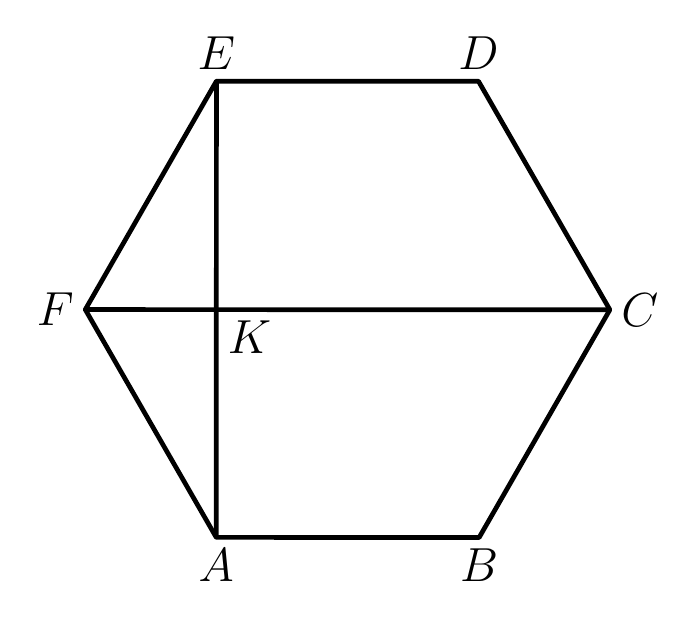
\begin{tikzpicture}[line join=round, line width=1.7pt]
  % Vertices (converted from pixels)
  \coordinate (F) at (-3.3489953273628594,0.01520830506354418);
  \coordinate (E) at (-1.6835854688313723,2.916246442094563);
  \coordinate (D) at (1.6446196556465744,2.9150046049115286);
  \coordinate (C) at (3.3132214582140422,0.012722464132372116);
  \coordinate (B) at (1.6531551925180166,-2.8790074737637448);
  \coordinate (A) at (-1.685747359223452,-2.8777616451010863);
  \coordinate (K) at (-1.6846681509609485,0.014587302662823967);

  % Hexagon sides
  \draw (F) -- (E) -- (D) -- (C) -- (B) -- (A) -- cycle;
  % Interior segments through K
  \draw (F) -- (C);
  \draw (E) -- (A);

  % Labels
  \node[above, font=\fontsize{17}{20.4}\selectfont] at (E) {$E$};
  \node[above, font=\fontsize{17}{20.4}\selectfont] at (D) {$D$};
  \node[right, font=\fontsize{17}{20.4}\selectfont] at (C) {$C$};
  \node[left, font=\fontsize{17}{20.4}\selectfont] at (F) {$F$};
  % K label: lower-right of the intersection (north west anchor at K)
  \node[anchor=north west, font=\fontsize{17}{20.4}\selectfont] at (K) {$K$};
  \node[below, font=\fontsize{17}{20.4}\selectfont] at (A) {$A$};
  \node[below, font=\fontsize{17}{20.4}\selectfont] at (B) {$B$};
\end{tikzpicture}
\end{document}
% GEOAGENT_REPAIR_V1 c18a466396f54661 bffbdf1a7d92e833642f745ac2ca28ac166ba5e3e2ecfe1523138d77df306e1c
